\chapter{背景}
\label{chap:background}

\section{研究背景}

今日スマートフォンやタブレットなどのモバイルデバイスが普及している。
\begin{figure}
  \begin{center}
    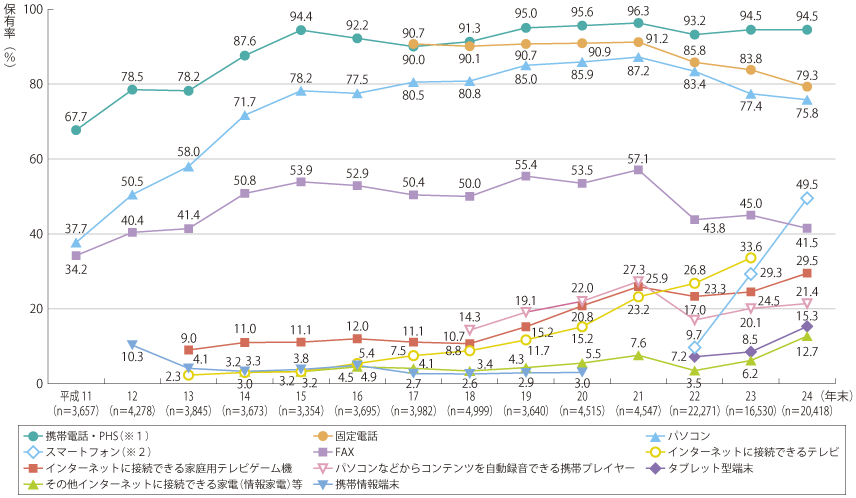
\includegraphics[width=14cm,bb=0 0 856 498]{images/internet.png}
    \caption{主な情報通信機器の普及状況(出典\cite{internet})}
    \label{internet}
  \end{center}
\end{figure}
それらを使う上で文字入力は欠かせない。
文字入力の機会は多い。
デバイスの能力はとても成長している。
でも文字入力に関してはほとんど成長していない。
文字入力にもデバイスに適したよりよいものがある。
文字入力のユーザの体験ももっと向上すべきである。
今回は日本人向けのシステムとして作った。

ユーザにはそれぞれコンテキストがある。
コンテキストによって入力したい単語は推測できるのではないか

\section{仮説}
機械学習すれば計算することはできる。
集合知を使えばデータを集めることができる
